\documentclass{beamer}

\usepackage[english]{babel}
\usepackage{graphicx,ru}

% The title of the presentation:
%  - first a short version which is visible at the bottom of each slide;
%  - second the full title shown on the title slide;
\title[Finding differential trails using an evolutionary algorithm]{
Finding differential trails using an evolutionary algorithm}

% The author(s) of the presentation:
%  - again first a short version to be displayed at the bottom;
%  - next the full list of authors, which may include contact information;
\author[Tim van Dijk]{Tim van Dijk\texorpdfstring{\\ tim.vandijk96@gmail.com}{}}

% The institute:
%  - to start the name of the university as displayed on the top of each slide
%    this can be adjusted such that you can also create a Dutch version
%  - next the institute information as displayed on the title slide
\institute[Radboud University Nijmegen]{
  Institute for Computing and Information Sciences -- Digital Security \\
  Radboud University Nijmegen}

% Add a date and possibly the name of the event to the slides
%  - again first a short version to be shown at the bottom of each slide
%  - second the full date and event name for the title slide
\date[Lunch colloquium 7 dec 2018]{
  Lunch colloquium \\
  December 7, 2018}

\begin{document}

\begin{frame}[plain]
  \titlepage
\end{frame}

\begin{frame}
  \frametitle{Outline}
  \tableofcontents
\end{frame}

% Section titles are shown in at the top of the slides with the current section 
% highlighted. Note that the number of sections determines the size of the top 
% bar, and hence the university name and logo. If you do not add any sections 
% they will not be visible.
\section{Background information}
\begin{frame}
\frametitle{Research internship}
\begin{itemize}
    \item Part of the TRU/e master.
    \item 2.5 days a week for one semester.
    \item Supervised by Joan Daemen.
    \item Overarching theme: cryptography over GF($P$)
    \begin{itemize}
        \item Bitsliced $+, \cdot$ and $^2$ over GF(3), GF(5) and GF(7) for ARM.
        \item Multidimensional discrete Fourier transform with full precision.
        \item Finding MAC collisions though differential cryptanalysis.
        \item Key recovery after finding a collision.
    \end{itemize}
\end{itemize}
\end{frame}

%What
\begin{frame}{Cryptography in GF($P$) - What?}
\begin{itemize}
    \item Normally, in symmetric cryptography we work over GF(2).
    \item Here, we work over a Galois Field of size $P$ with $P$ a prime.
    \item This means we work with digits in $\{0, ..., P-1\}$ instead of bits that are either 0 or 1.
    \item In GF($P$) things often behave a little differently, for example addition no longer is the same as subtraction.
\end{itemize}
\end{frame}

%Why
\begin{frame}{Cryptography over GF($P$) - Why?}
\begin{itemize}
    \item Not only functions over GF(2) and GF($2^n$) have been studied extensively.
    \item Interesting differences that to a certain extent provide richer functionality than binary fields.
    \begin{itemize}
        \item GF($P$): Perfect Nonlinear Functions.
        \item GF(2): Almost Perfect Nonlinear Functions.
    \end{itemize}
    \item Try to capitalize on the large amount of theoretical results over GF($P$).
    % Er is eigenlijk veel theorie over die functies, maar niemand gebruikt ze in crypto
    \item Generalization might give new insights.
    \item Applicable to coding theory and signal modulation techniques?
\end{itemize}
\end{frame}

%How
\begin{frame}{Cryptography over GF($P$) - How?}
\begin{itemize}
    \item Specialized hardware - ternary computers are virtually nonexistent, but again, it might be useful in telecommunications.
    \item In practice, most data will continue to be represented in bit strings.
    \item Software emulation - $\lceil \log_{2}{P} \rceil$ bits required to store a digit in GF($P$).
\end{itemize}
\centering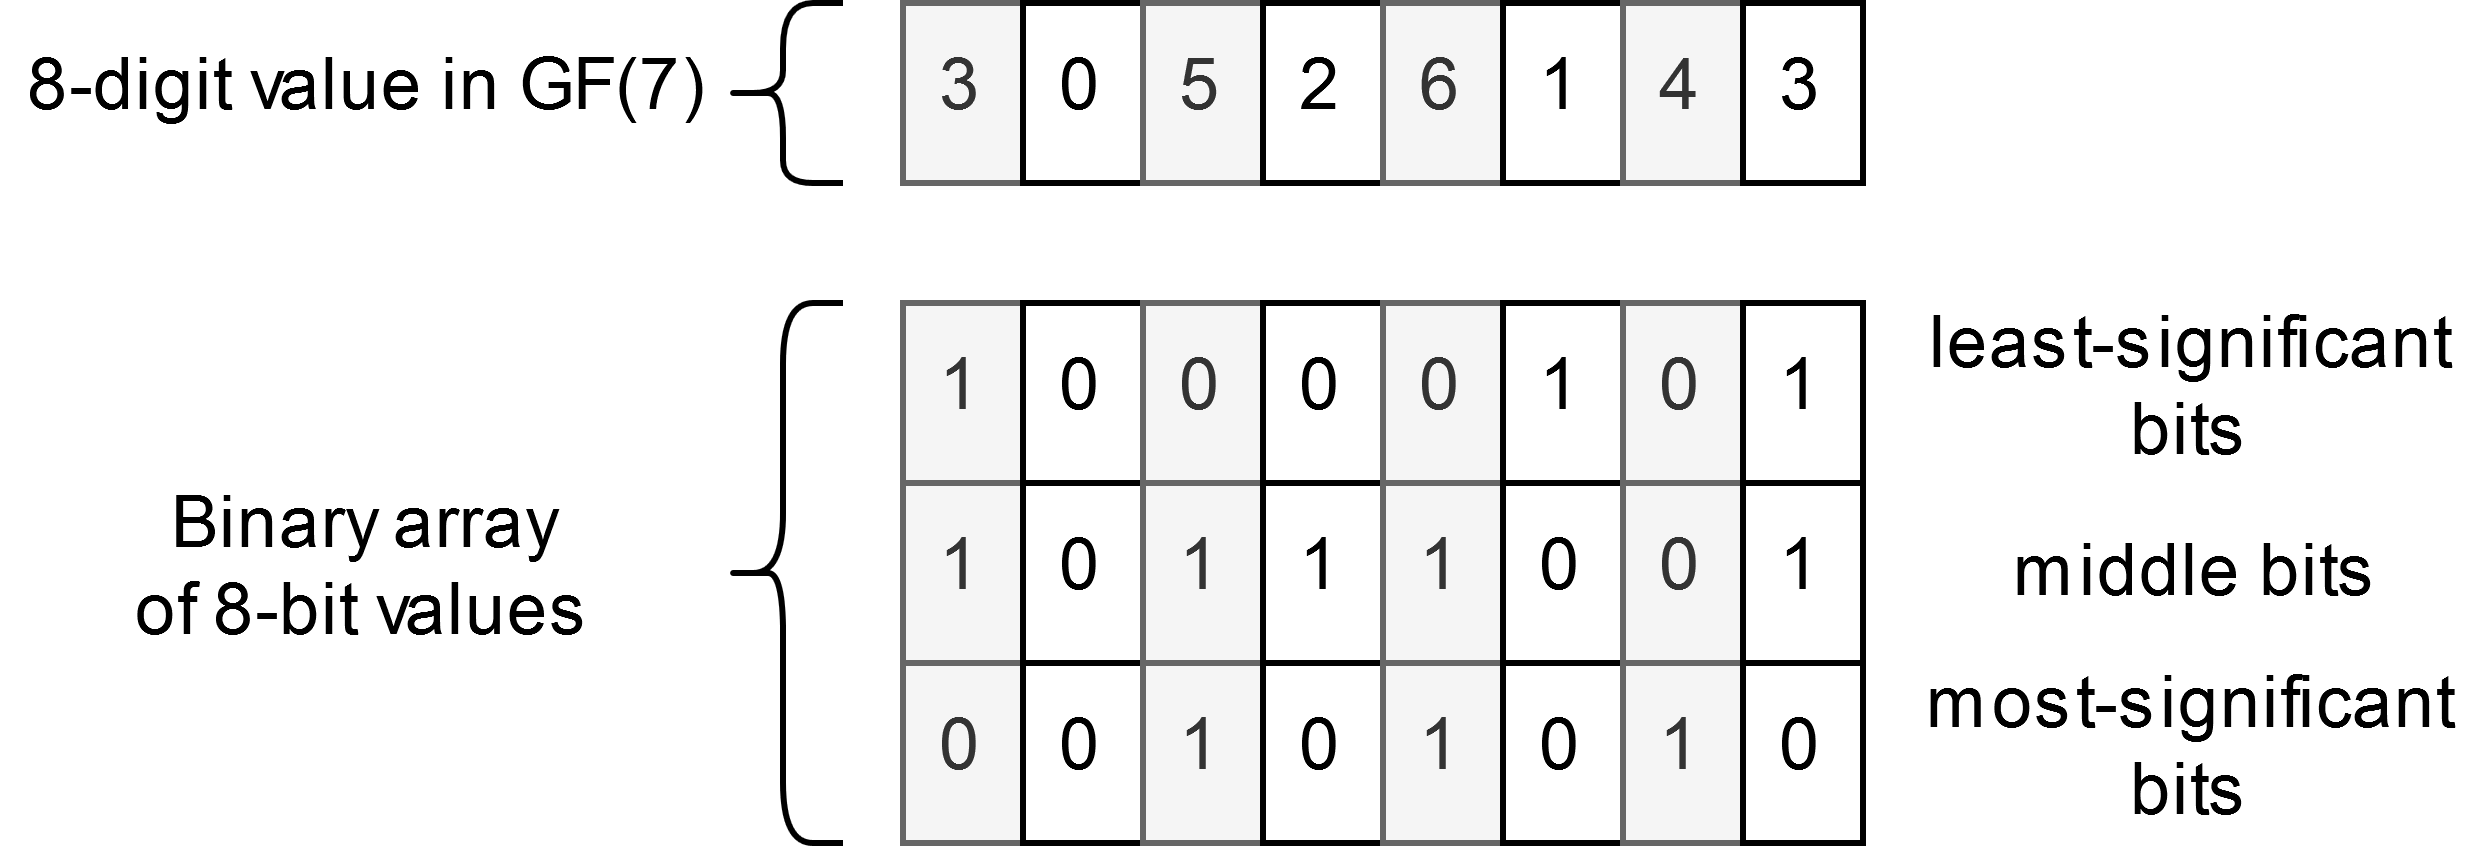
\includegraphics[scale=0.12]{encoding.png}
\end{frame}

\begin{frame}{Bitsliced operations for ARM}
Bitslicing is a technique where a computation is:
\begin{enumerate}
    \item reduced to elementary operations (e.g. OR, AND, XOR);
    \item executed in parallel, with as many simultaneous instances a there are bits in a register.
\end{enumerate}
To work, data needs to be transposed:
\begin{table}[]
\begin{tabular}{llll || llll}
Normal & & & & Bitsliced & & & \\ \hline
$r_0$ & $a_2$ & $a_1$ & $a_0$ & $r_0$ & $c_0$ & $b_0$ & $a_0$ \\ \hline
$r_1$ & $b_2$ & $b_1$ & $b_0$ & $r_1$ & $c_1$ & $b_1$ & $a_1$ \\ \hline
$r_2$ & $c_2$ & $c_1$ & $c_0$ & $r_2$ & $c_2$ & $b_2$ & $a_2$ \\ \hline
\end{tabular}
\end{table}
\end{frame}

\begin{frame}[fragile=singleslide]{Bitsliced operations for ARM}
\begin{table}[]
\begin{tabular}{llll || llll}
Normal & & & & Bitsliced & & & \\ \hline
$r_0$ & $a_2$ & $a_1$ & $a_0$ & $r_0$ & $c_0$ & $b_0$ & $a_0$ \\ \hline
$r_1$ & $b_2$ & $b_1$ & $b_0$ & $r_1$ & $c_1$ & $b_1$ & $a_1$ \\ \hline
$r_2$ & $c_2$ & $c_1$ & $c_0$ & $r_2$ & $c_2$ & $b_2$ & $a_2$ \\ \hline
\end{tabular}
\end{table}

For values a, b and c, compute in parallel: $X_0 + X_0 \cdot X_1$. 
\begin{verbatim}
AND    R3, R0, R1    ; R3 := X0 * X1
EOR    R3, R0, R4    ; R3 := X0 + (X0 * X1)
\end{verbatim}
Can sometimes be used to dramatically increase throughput at the cost of increased latency.
\end{frame}

\begin{frame}{Bitsliced operations for ARM}
\begin{itemize}
    \item Addition, multiplication and squaring in GF(3), GF(5) and GF(7).
    \item Represent the output in terms of a function of the input bits.
    \item Difficult to do by hand $\rightarrow$ use logic synthesis tools.
    \item Implemented in assembly for ARM Cortex M4.
\end{itemize}
\end{frame}

\begin{frame}{Multidimensional discrete Fourier transform}
\begin{itemize}
    \item GF($P$) version of the Walsh-Hadamard transform.
    \item Important in linear cryptanalysis.
    \item Used to compute the correlation of a function with all linear functions at once.
    \item In the binary case, correlation is between $-1$ and $1$.
    \item In the non-binary case, it deals with complex numbers.
    \item Two versions: 
    \begin{itemize}
        \item a straightforward one that uses floating points. Numbers are represented as $a + bi$. 
        \item one that uses polynomials of form $\sum a_j\omega^j$ with $\omega = e^{\frac{2\pi i}{p}}$
    \end{itemize} 
    \item The latter has full precision.
\end{itemize}
\end{frame}

\begin{frame}{MACs using (round reduced) transformations}
\centering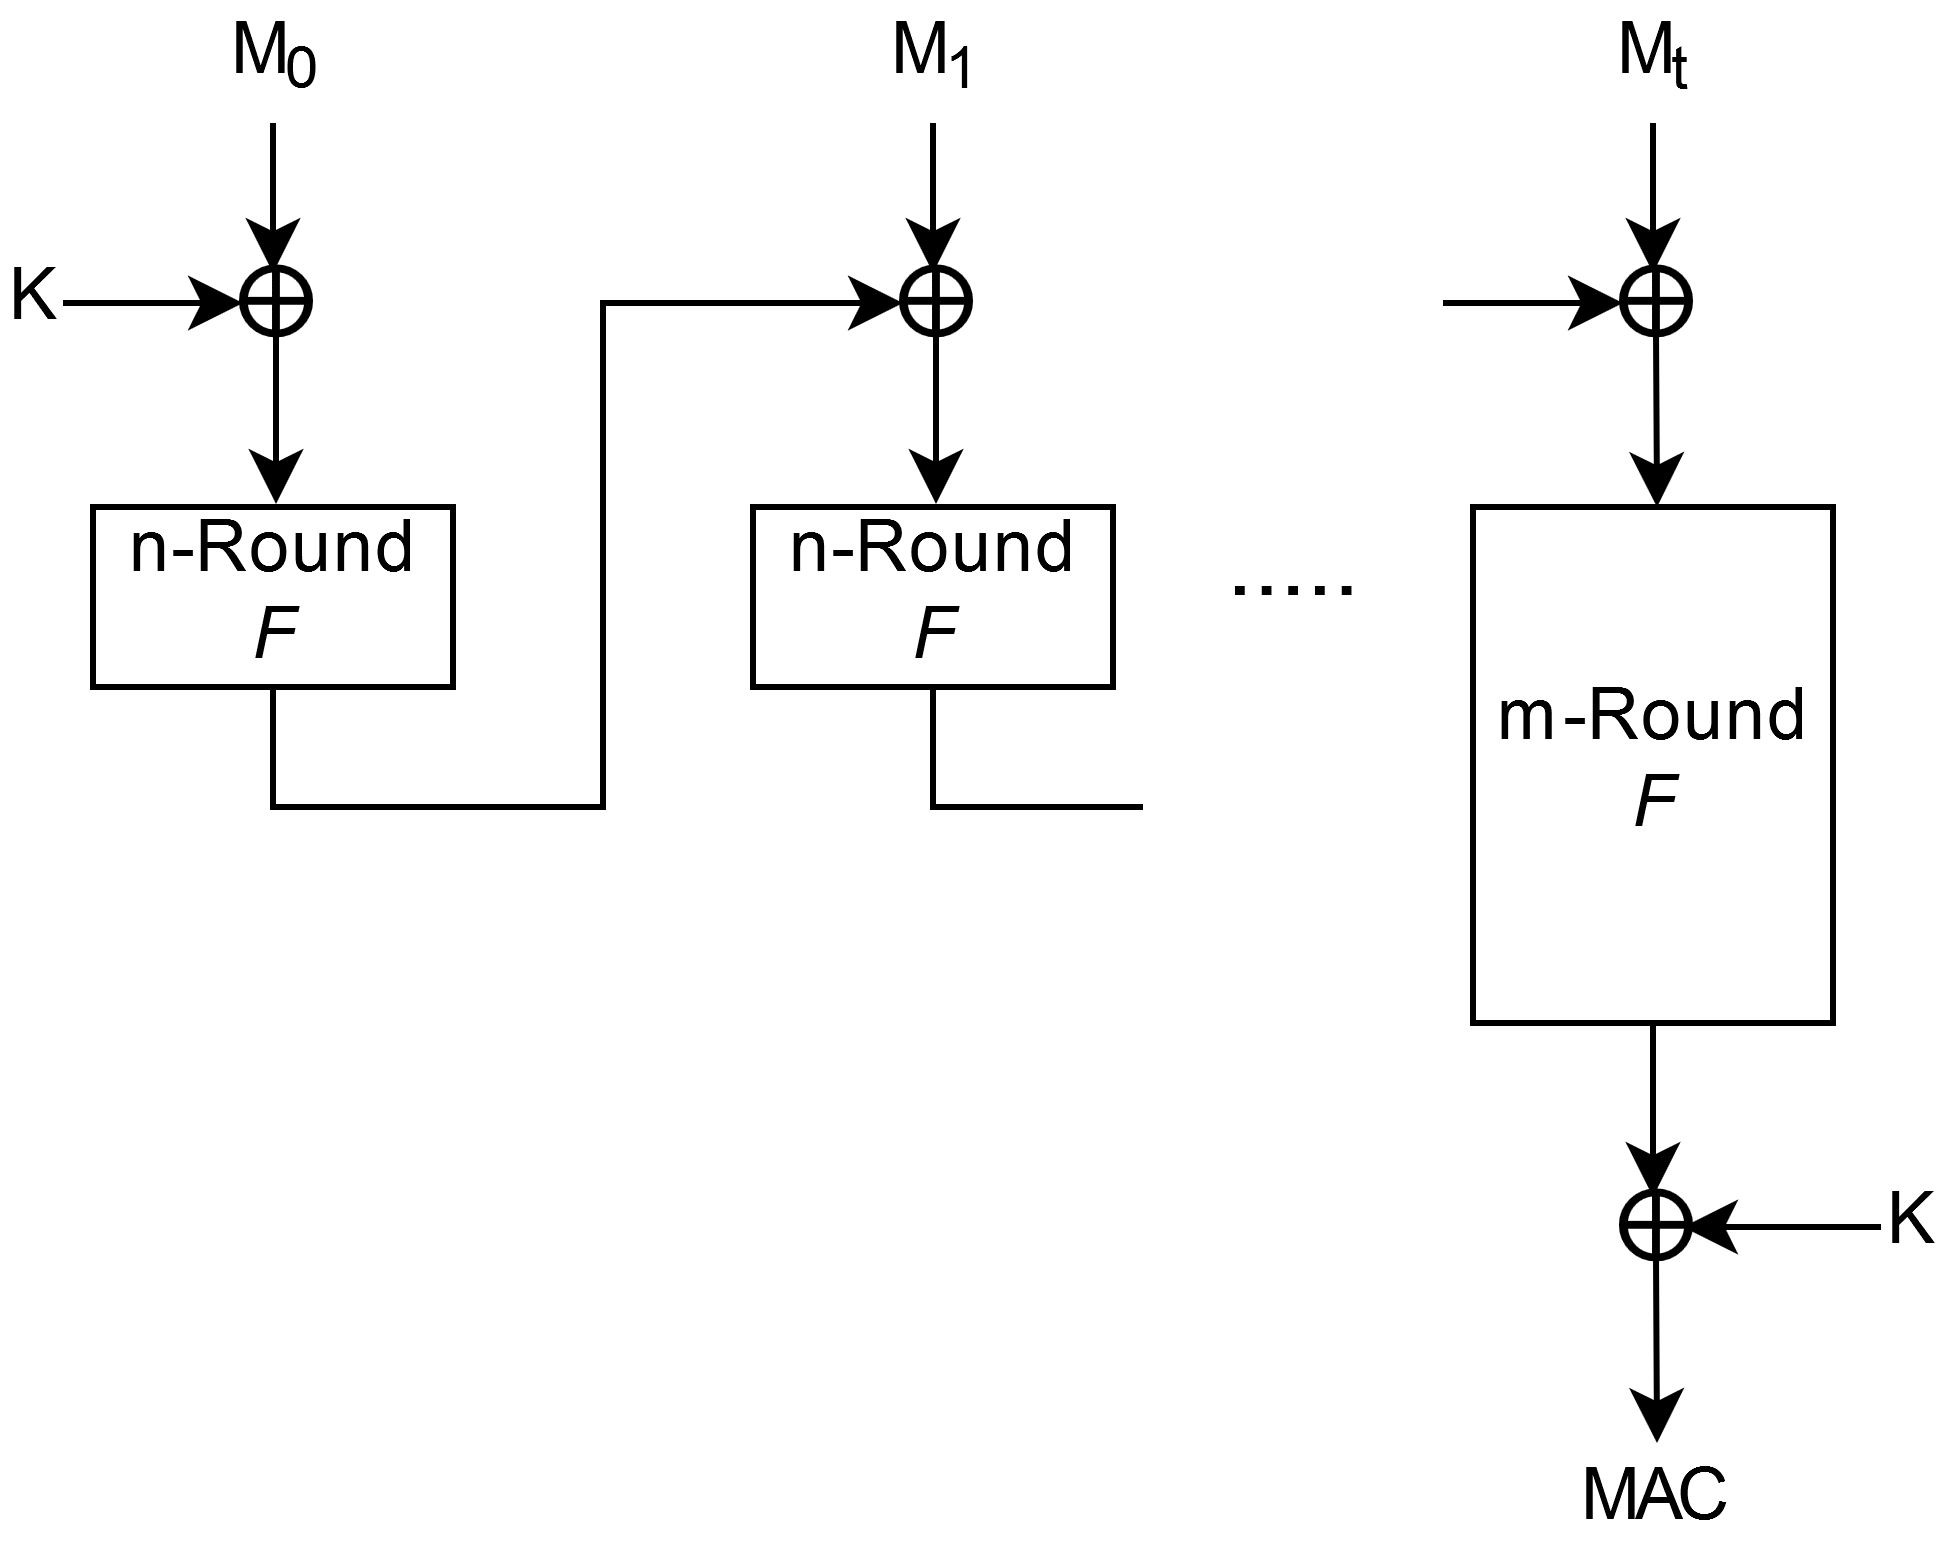
\includegraphics[scale=0.12]{HMAC_HighResV2.png}
\end{frame}

\begin{frame}{The cryptographic transformation ThreeCircle}
\begin{itemize}
    \item A permutation designed by Joan for me to experiment on.
    \item Operates on a state of 160 digits over GF(3).
    \item State $a$ arranged in 5 32-digit lanes, we write $a = (a_0, a_1, a_2, a_3, a_4)$.
    \item Classical iterated structure: it iterates a round function $R_i$ 12 times to the state.
\end{itemize}
\end{frame}

\begin{frame}{MACs using (round reduced) ThreeCircle}
\centering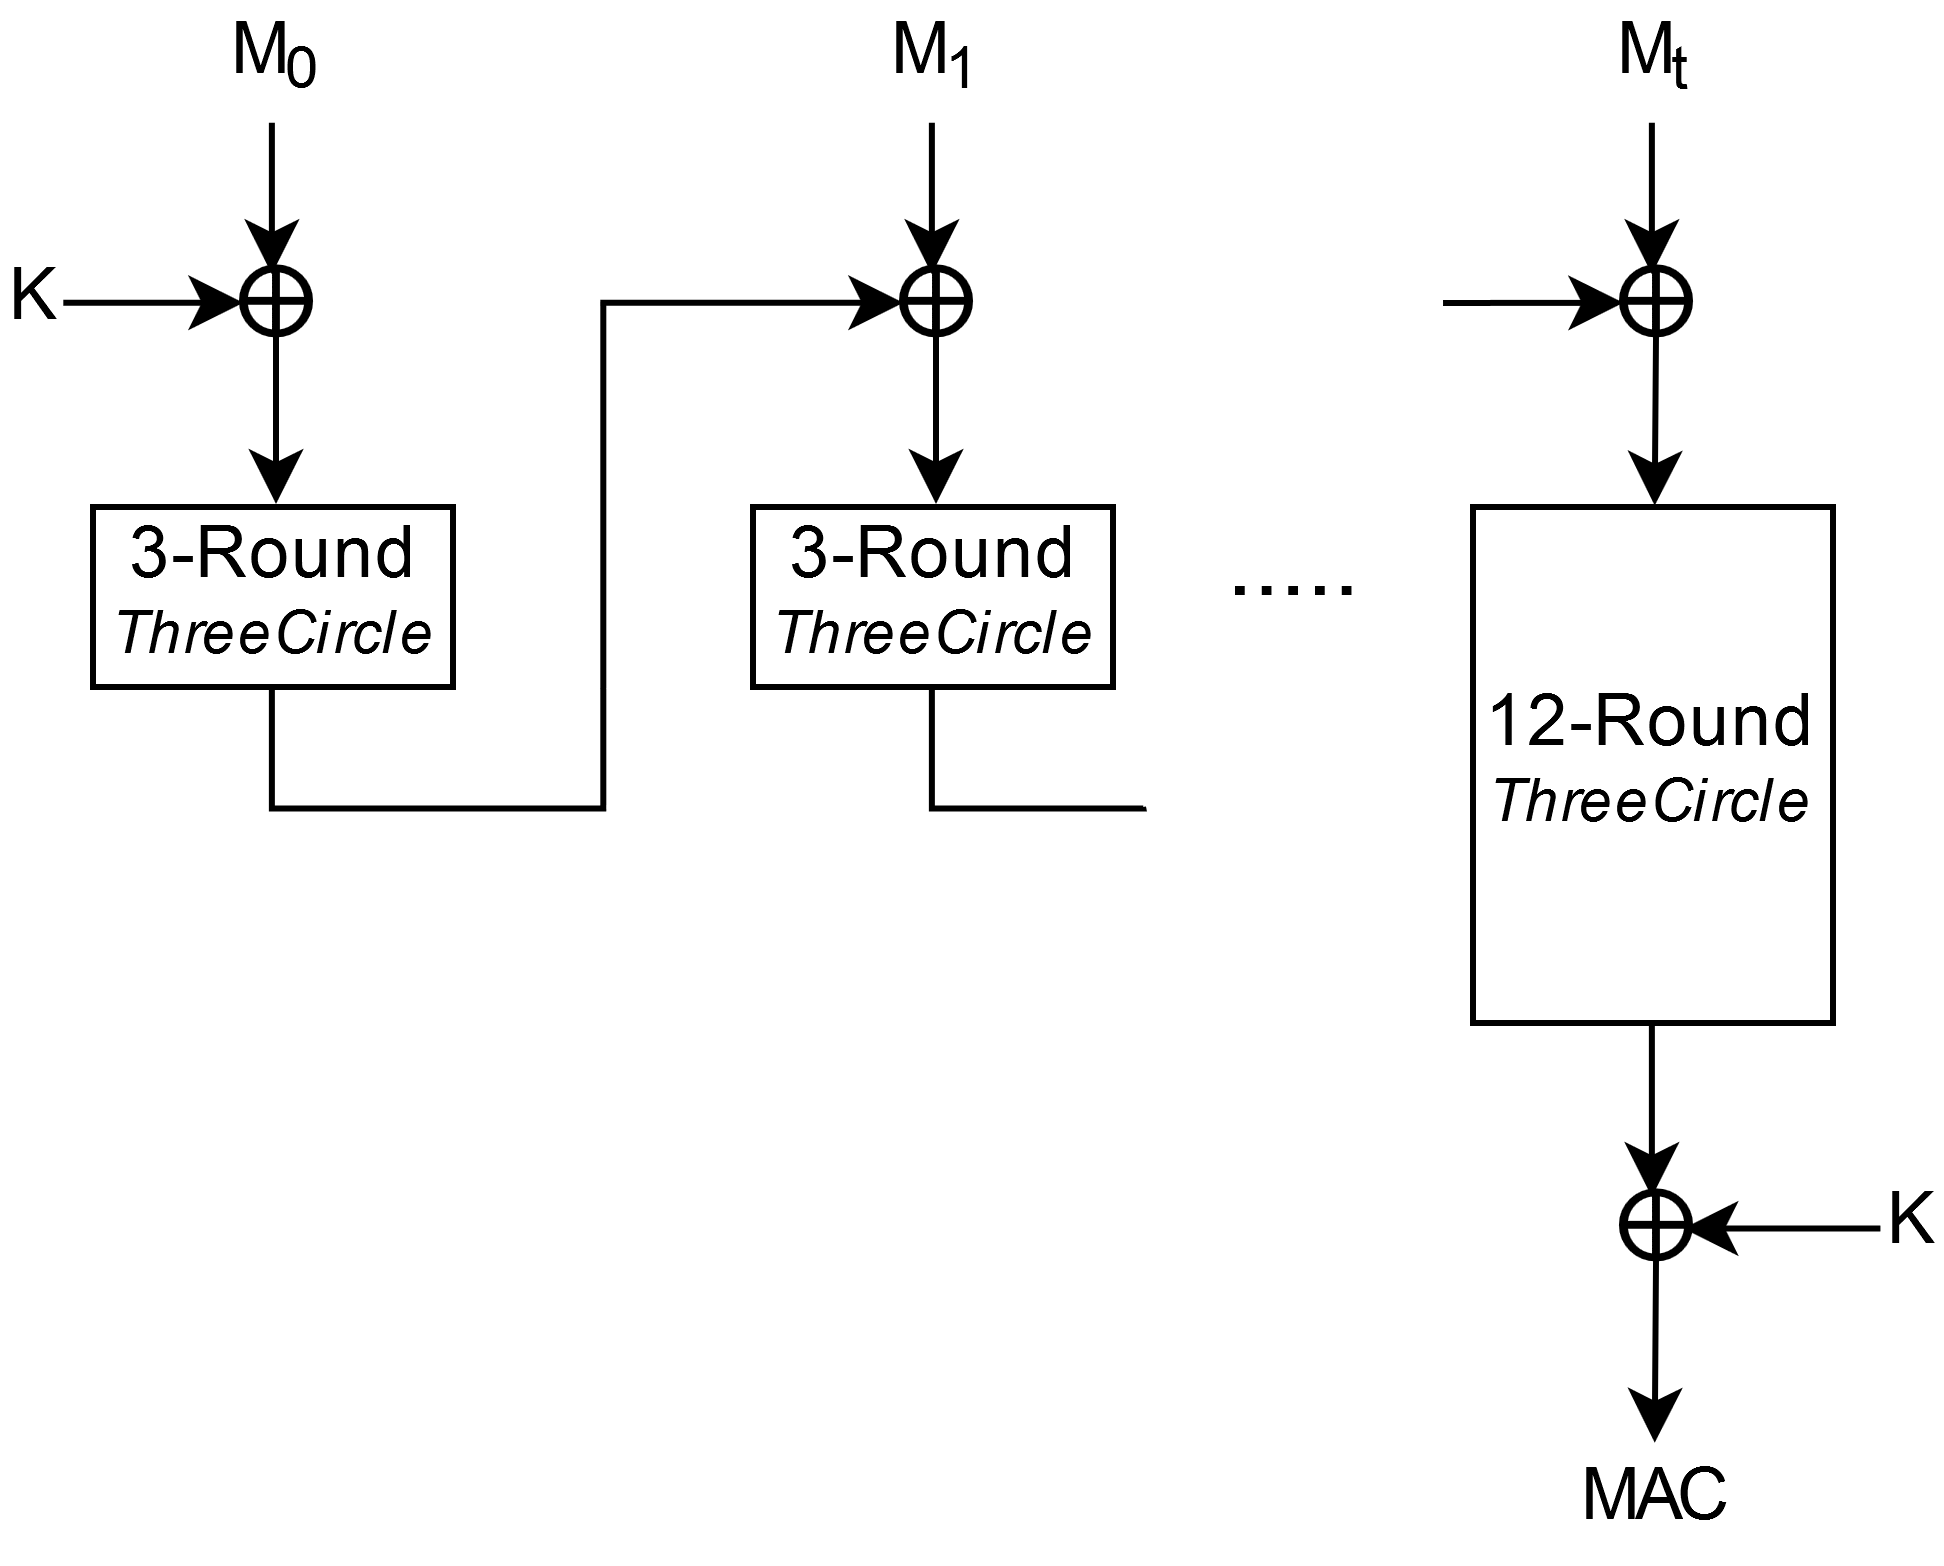
\includegraphics[scale=0.12]{HMAC_HighRes_ThreeCircle.png}
\end{frame}

\begin{frame}{The round function of ThreeCircle}
\begin{block}{Non-linear step $\chi$}
\begin{itemize}
    \item $a_y \leftarrow a_y + a_{y+1}a_{y+1}\lll 1 \text{ for all } y \text{ in parallel}$
\end{itemize}
\end{block}
\begin{block}{Mixing step $\theta$}
\begin{itemize}
    \item $p \leftarrow a_0 + a_1 + a_2 + a_3 + a_4$
    \item $e \leftarrow p \lll 12 + p \lll 17$
    \item $a_y \leftarrow a_y + (e \lll y) \text{ for all } y$
\end{itemize}
\end{block}
\begin{block}{Transposition step $\pi$}
\begin{itemize}
    \item $a_y \leftarrow a_{y+1} \text{ for all } y \text{ in parallel}$
\end{itemize}
\end{block}
\begin{block}{Transposition step $\rho$}
\begin{itemize}
\item $a_y \leftarrow a_y \lll r_y \text{ for all } y \text{ with } r = (0, 2, 6, 11, 19)$
\end{itemize}
\end{block}
\end{frame}
 
\begin{frame}{Differential cryptanalysis}
\begin{itemize}
    \item The study of how differences in information input can affect the resultant difference at the output.
    \item We want to use it to find colliding MACs.
    \item Trail: knowledge of how an input difference propagates and the probability of it happening.
    \item Differential: same as trail, but we do not care about the difference between each round.
\end{itemize}
\end{frame}

\begin{frame}{Differential cryptanalysis - Differentials}
\begin{itemize}
    \item Assume we have the following differential: $(\Delta_{in}, \Delta_{out})$ with associated differential probability $DP(\Delta_{in}, \Delta_{out}) = p$.
    \item We start with two messages such that $\Delta_{in} = M_1 - M_0 = (M_1 + K) - (M_0 + K)$
    \item With probability $p = DP(\Delta_{in}, \Delta_{out})$, we have that: $\Delta_{out} = F(M_1 + K) - F(M_0 + K) = (F(M_1 + K) + K) - (F(M_0 + K) + K)$
\end{itemize}
\centering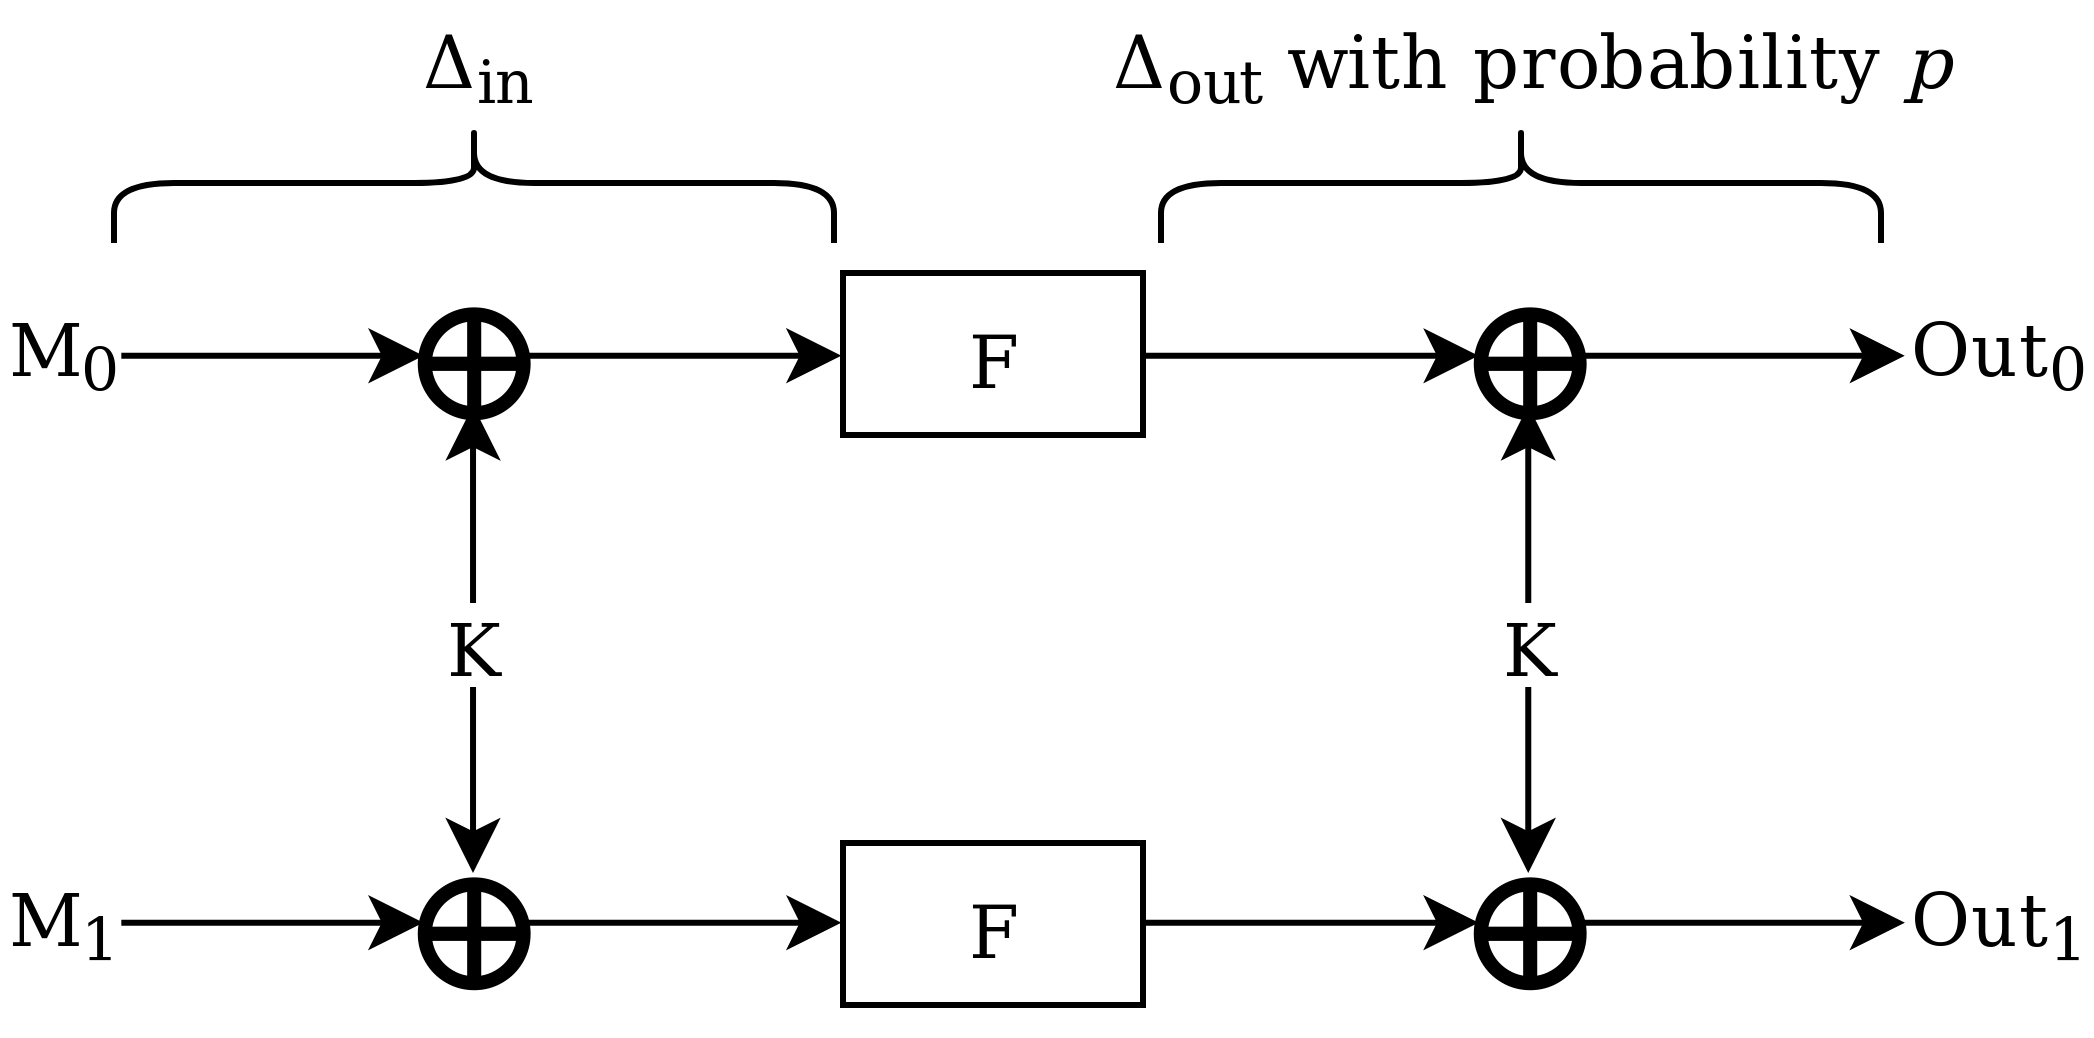
\includegraphics[scale=0.101]{Differential_Example.png}
\end{frame}

\begin{frame}{Differential cryptanalysis - Finding collisions}
%\begin{itemize}
%    \item To find a collision:
%    \begin{enumerate}
%        \item Randomly pick $X = X_0 || X_1$.
%        \item Set $Y_0 = X_0 + \Delta_{in}$.
%        \item Compensate for $\Delta_{out}$ by setting $Y_1 = X_1 - \Delta_{out}$.
%        \item Compute $MAC(X)$ and $MAC(Y)$ hoping they are the same.
%        \item Repeat above steps on average $p$ times until the MACs collide.
%    \end{enumerate}
%\end{itemize}
\centering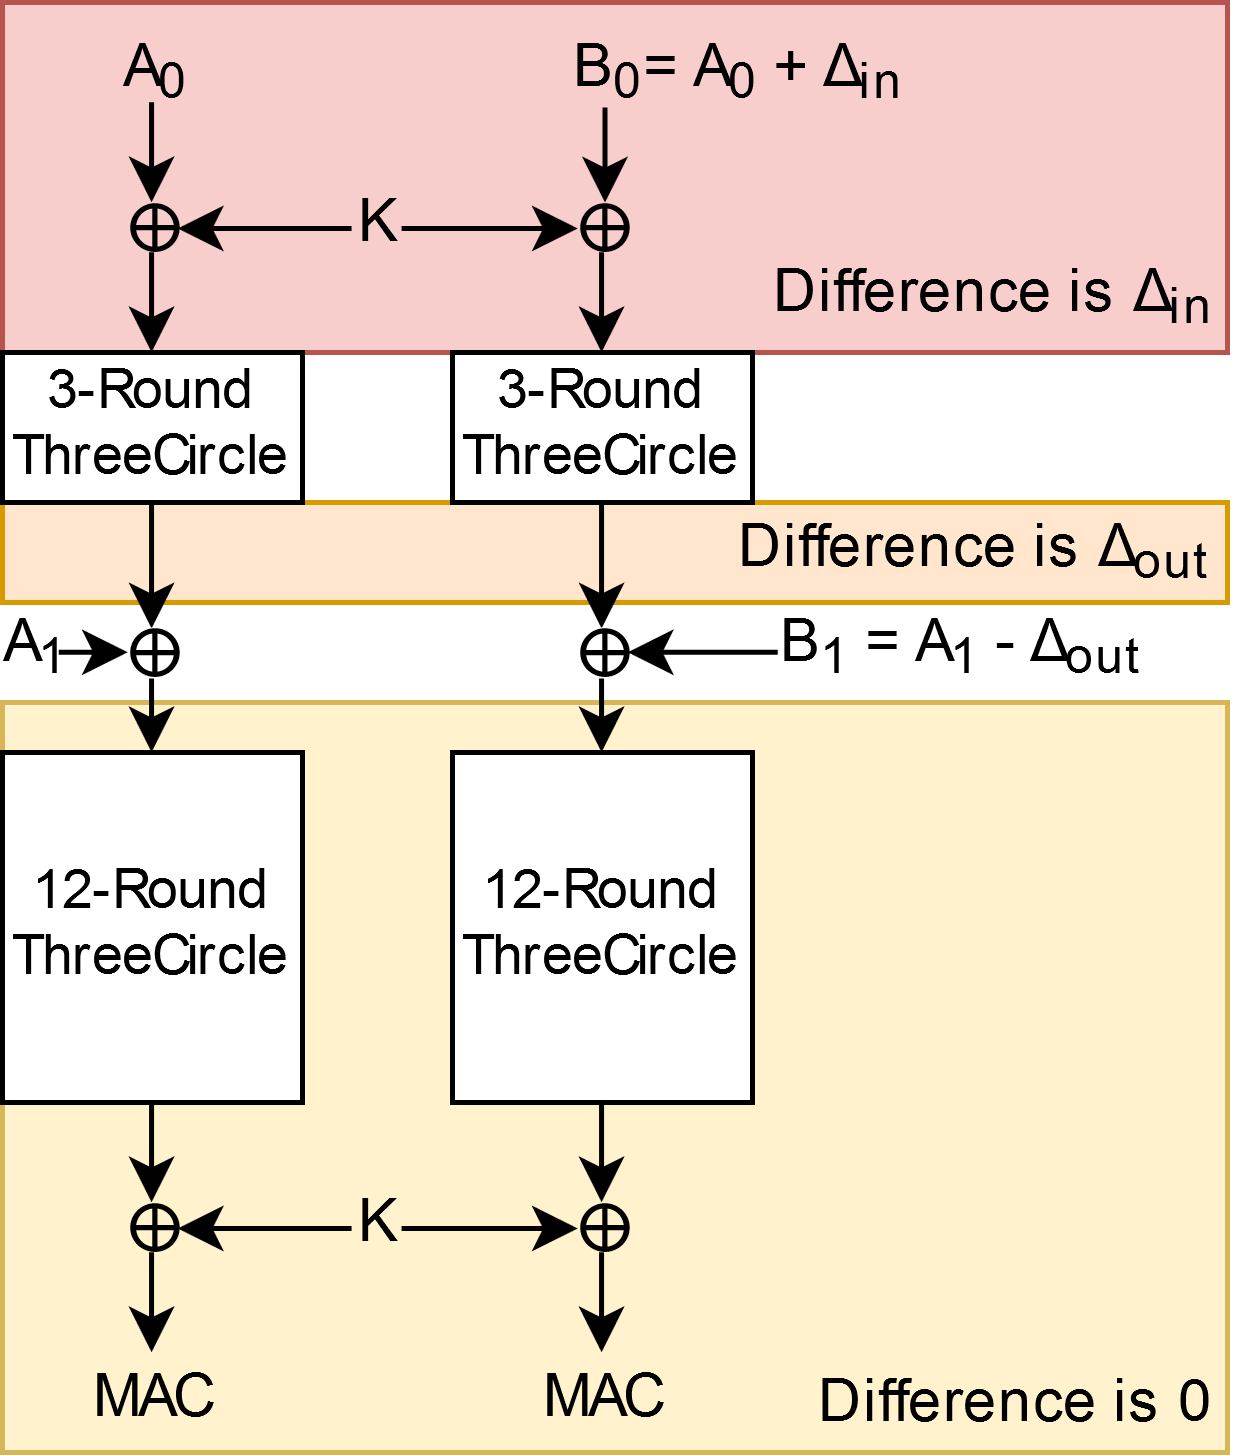
\includegraphics[scale=0.145]{Collision.png}
\end{frame}

\begin{frame}{How do differences propagate in ThreeCircle?}
\begin{block}{Non-linear layer}
\begin{itemize}
    \item Each non-zero digit in the differential causes 3 equally likely branches.
    \item Branches lower the differential probability.
\end{itemize}
\end{block}

\begin{block}{Mixing layer}
\begin{itemize}
    \item Only has effect when there are non-zero digits in differential of the parities.
    \item Does not cause branching, but causes diffusion (i.e. more non-zero digits in the differential).
\end{itemize}
\end{block}

\begin{block}{Transposition layer}
\begin{itemize}
    \item Moves the digits around.
    \item Does not cause branching, but spreads the active digits.
\end{itemize}
\end{block}
\end{frame}

\section{Finding trails}

\begin{frame}{Finding trails}
\begin{itemize}
\item Finding best trails is an open problem.
\item Finding a trail that spans 1 round often is doable by hand.
\item Finding a trail that spans multiple rounds gets \emph{very} complex \emph{very} fast.
\item Essentially an optimization problem: we want to find an input/output difference that has an as high as possible differential probability.
\item Problem: search space is \emph{huge}.
\end{itemize}
\end{frame}

\begin{frame}{Evolutionary algorithms}
\begin{itemize}
    \item An evolutionary algorithm (EA) is a generic population-based optimization algorithm.
    \item An EA uses mechanisms inspired by biological evolution, such as reproduction, mutation, recombination and selection.
    \item Candidate solutions play the role of individuals in a population, and the fitness function determines the quality of the solutions.
    \item It often works well on NP-problems.
    \item Based on underlying assumptions that are not necessarily true, most notably the building block hypothesis.
\end{itemize}
\end{frame}

\begin{frame}{Evolutionary algorithms - Implementation}
\begin{enumerate}
    \item Generate the initial population of individuals randomly.
    \item Evaluate the fitness of each individual.
    \item Repeat until termination:
    \begin{itemize}
        \item Select the best-fit individuals for reproduction.
        \item Breed new individuals through crossover and mutation.
        \item Evaluate the individual fitness of new individuals.
        \item Replace least--fit population with new individuals.
    \end{itemize}
\end{enumerate}
\end{frame}

\begin{frame}{Evolutionary algorithms - fitness function}
\begin{itemize}
    \item Many design decisions when implementing an EA.
    \item Perhaps the most important one is the fitness function.
    \item Single figure of merit that summarizes how close a solution is to achieving a set of aims.
    \item If chosen poorly, the algorithm will converge on a poor solution or not at all.
    \item We want to minimize the number of branches $\rightarrow$ minimize the number of active digits going into $\chi$.
    \item Use sum of weights going to $\chi$. Problem: noisy.
\end{itemize}
\end{frame}

\begin{frame}{Evolutionary algorithms - Tweaks to make things work}
\begin{itemize}
    \item The fitness function is noisy since many trails are possible for a given $\Delta_{in}$, therefore I run the fitness function many times and return weight of best trail.
    \item Empirically, I know $\Delta_{in}$'s of good trails tend to have most digits set to 0, so to speed up the process I create the initial population such that most digits are 0.
\end{itemize}
\end{frame}

\section{Results}

\begin{frame}{Results}
\begin{itemize}
    \item I could not find a good trail for 3 round ThreeCircle by hand.
    \item We anticipated that the best trail would have a DP of $\frac{1}{3^{26}}$.
    \item I used an EA to find a trail with DP $\frac{1}{3^{16}}$.
    \item The trail I found should not exist and reveals a weakness in (the rotation constants of) ThreeCircle.
\end{itemize}
\end{frame}

\section{Conclusion}
\begin{frame}{Conclusion}
\begin{itemize}
    \item It might be worth pursuing the use of evolutionary algorithms to find trails for differential cryptanalysis.
\end{itemize}
\end{frame}

\end{document}
